\documentclass[11pt,letterpaper]{article}
\usepackage{../packagesComp}
\usepackage{../optionsComp}

\input{../macrosComp}

\title{Compiladores 2023-2\\ Facultad de Ciencias UNAM \\ Tarea 6}
\author{Lourdes Gonz\'alez Huesca\\ Juan Alfonso Gardu\~no Sol\'is \and  
Braulio Aaron Santiago Carrillo  \\Ma. Fernanda Mendoza Castillo}
\date{Entrega: \textbf{lunes 29 mayo 2023}~\footnote{Entrega en la 
plataforma classroom del grupo, en equipos de dos o tres personas.}}


\begin{document}

\maketitle
\begin{enumerate}
\begin{multicols}{2}
\item Varios lenguajes de programaci\'on, por ejemplo \textsc{C}, tienen 
definido el enunciado \texttt{switch}:
\begin{verbatim}
switch E
   begin
      case V1 : S1
      case V2 : S2
      ...
      case Vn−1 : Sn−1
   default: Sn
end
\end{verbatim}
Describe una forma de traducir este enunciado a c\'odigo de tres direcciones 
(puedes usar saltos y condicionales).
Explica y justifica que el c\'odigo de tres direcciones propuesto respeta el 
mismo comportamiento que el \texttt{switch}.


\item Considera el siguiente c\'odigo:
\begin{verbatim}
int mul(int x, int y) {
if (x) return y - (0 - mul(x + 1, y)); 
   else return 0; }
\end{verbatim}
Proporciona una traducci\'on a RTL suponiendo que ya se han seleccionado 
las instrucciones. \\Deber\'as mostrar las traducciones intermedias de 
subexpresiones del c\'odigo.
\columnbreak
\item 
Utilizando la tabla de traducci\'on entre una representaci\'on 
intermedia lineal y las instrucciones de arquitectura MIPS, 
genera el c\'odigo m\'aquina para la siguiente secuencia:
\begin{minted}[escapeinside=//]{c}
 d := c + 8
 a := a + b/$^{last}$/
 M[d/$^{last}$/] := a
 IF a < c THEN L1 ELSE L2
 LABEL L1
\end{minted}

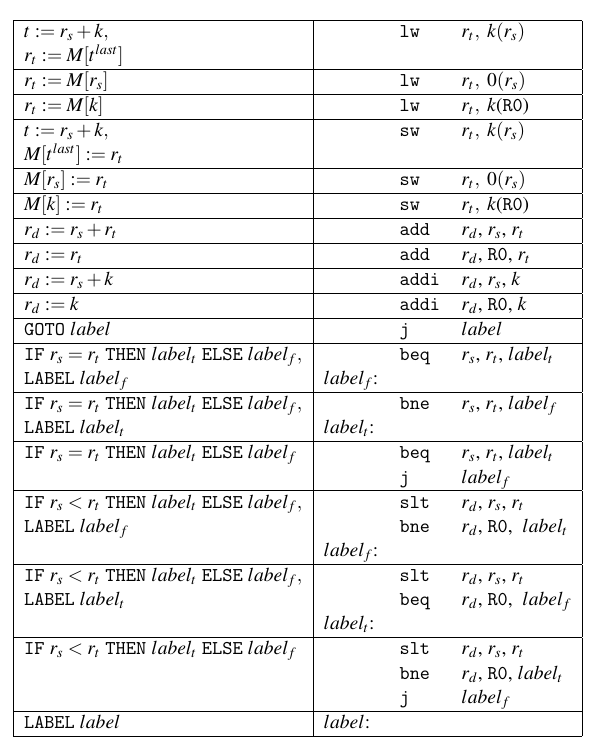
\includegraphics[width=.45\textwidth]{../../imagenes/MIPSInstrSet}

\end{multicols}

\newpage

\item \textbf{Hasta 1.5pts extra.} Determina el código de tres direcciones
de la siguiente expresión,
\begin{center}
   $(a \ SUB \ b ) \ MOD \ ((MINUS \ c)  \ SUB \ d)$
\end{center}
usando las reglas semánticas siguientes. \\
Pueden omitir la explicación de la creación del árbol de sintaxis abstracta, 
pero hay que explicar los pasos del análisis semántico.

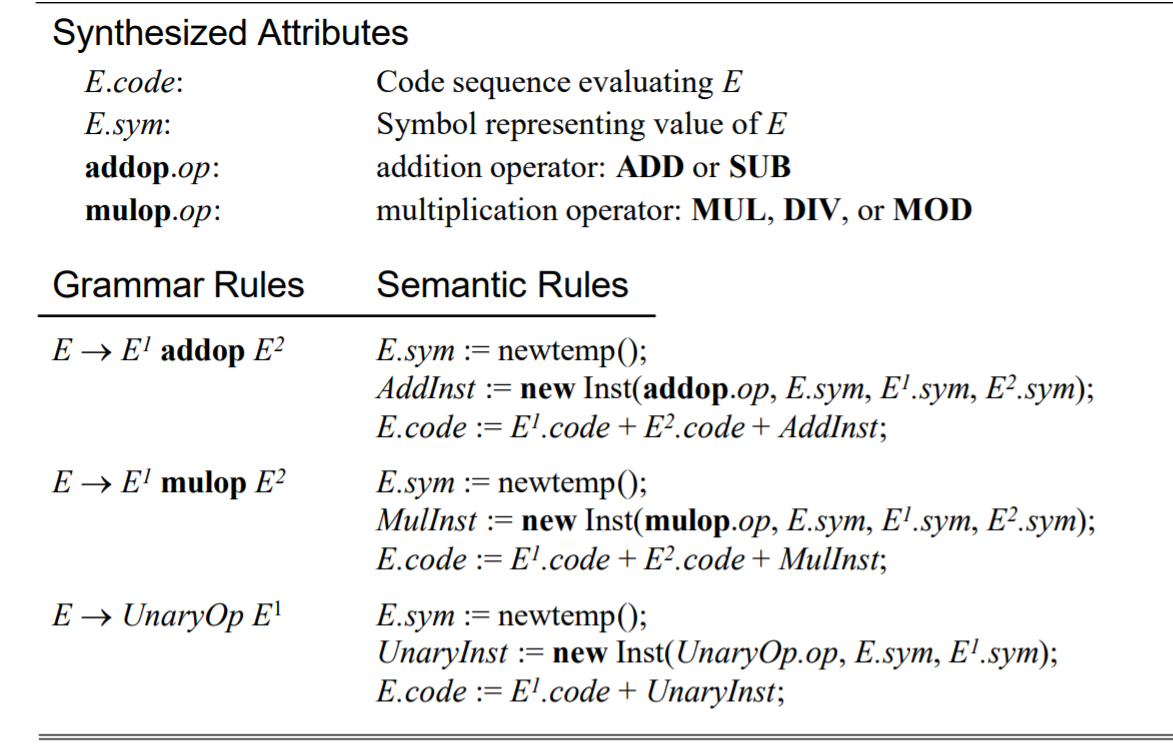
\includegraphics[width=0.6\linewidth]{../../imagenes/Fun_Sem_1.PNG}
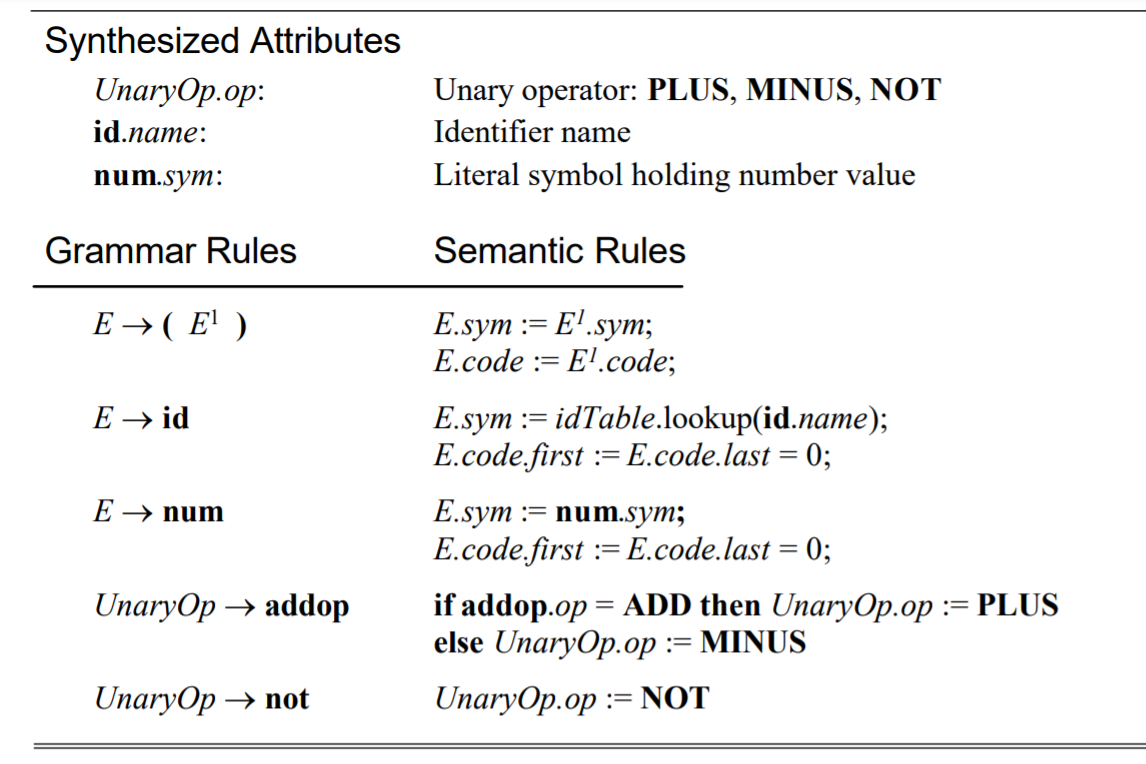
\includegraphics[width=0.6\linewidth]{../../imagenes/Funciones_Semanticas_2.PNG}

\end{enumerate}


\end{document}
